\chapter{\ifenglish Background Knowledge and Theory\else ทฤษฎีที่เกี่ยวข้อง\fi}

\textbf{บทนำ}
\begin{mypara}
\indent ในบทนี้จะนำเสนอการศึกษาทฤษฎีและงานวิจัยที่เกี่ยวข้อง เพื่อเป็นแนวทางในการออกแบบและพัฒนาเว็บแอปพลิเคชันสำหรับระบบสนับสนุนการตัดสินใจในการวางแผนระบบขนส่งสาธารณะ 
    ระบบดังกล่าวถูกออกแบบให้ใช้การแบบจำลอง เพื่อสร้างสถานการณ์บนแผนต่างๆ 
    และให้ผลลัพธ์ใกล้เคียงกับความเป็นจริง ในบทนี้จะอธิบายแนวคิดและทฤษฎีที่เกี่ยวข้องกับการพัฒนาระบบดังกล่าว 
\end{mypara}

\section{ทฤษฎีและความรู้ที่เกี่ยวข้องในการทำแบบจำลอง}
    \begin{mypara}
        \indent ในส่วนนี้จะกล่าวถึงทฤษฎีและความรู้ที่เกี่ยวข้องกับการทำแบบจำลอง (Simulation) ที่ถูกใช้ในโครงงานนี้
        เพื่อให้เข้าใจถึงหลักการและแนวคิดที่นำมาใช้ในการพัฒนาระบบสนับสนุนการตัดสินใจในการวางแผนระบบขนส่งสาธารณะ
        โดยทั่วไปแล้วแบบจำลองนั้นมีหลายประเภท เราได้เลือกใช้ทฤษฎีและแนวคิดที่เหมาะสมกับการจำลองระบบขนส่งสาธารณะ ดังนี้
    \end{mypara}

\subsection{Queuing Theory}
\begin{mypara}
    \indent ทฤษฎีการรอคอย (Queuing Theory) เป็นศาสตร์ทางคณิตศาสตร์และวิศวกรรมที่ใช้ในการวิเคราะห์พฤติกรรมของระบบที่มี 
    “การรอคอย” หรือ “แถวคิว” เกิดขึ้น โดยทั่วไป ระบบคิวจะประกอบด้วย 3 ส่วนหลัก ได้แก่ ลูกค้า (Customers), 
    แถวรอ (Queue/Waiting Line) และ ผู้ให้บริการ (Server) เมื่อลูกค้ามาถึงระบบ หากมีผู้ให้บริการว่างก็จะได้รับบริการทันที 
    แต่ถ้าผู้ให้บริการไม่ว่าง ลูกค้าจะต้องเข้าไปอยู่ในแถวรอจนกว่าจะถึงคิว
\end{mypara}

\begin{figure}[h]
    \centering
    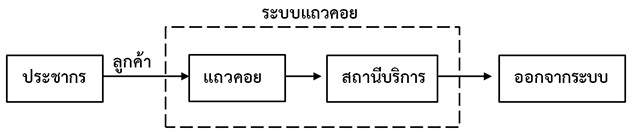
\includegraphics[width=0.75\textwidth]{Query_theory.png}
    \caption{กระบวนการแถวคอย}
    \label{fig:example}
\end{figure}
\indent ในระบบของเรา เรานำแนวคิด Queuing Theory มาประยุกต์ใช้กับการจำลองการเดินทางของผู้โดยสารและการให้บริการโดยรถบัส โดยใช้ Queue Discipline แบบ First in First out และสามารถอธิบายได้ดังนี้
\begin{enumerate}
    \item \textbf{Customers Arrivals (ผู้โดยสารมารอที่ป้าย):} ผู้โดยสารมาถึงป้ายรถตามอัตราการมาถึง (arrival rate) ซึ่งอาจเป็นแบบสุ่มหรือกำหนดเป็นช่วงเวลา
    \item \textbf{Waiting Line (แถวรอขึ้นรถ):} ผู้โดยสารรอรถอยู่ในแถวตามลำดับการมาถึง (FIFO) จนกว่ารถจะมาถึง
    \item \textbf{Server (รถบัส):} รถบัสทำหน้าที่ให้บริการผู้โดยสาร โดยสามารถรับผู้โดยสารได้ตามความจุของรถและเวลาที่ใช้ในการให้บริการ
    \item \textbf{Customer Leaves/Departure (ผู้โดยสารลงจากรถ):} ผู้โดยสารลงจากรถหลังสิ้นสุดการเดินทาง ทำให้พื้นที่ในรถว่างสำหรับผู้โดยสารใหม่
\end{enumerate}

\subsection{Simulation Model}
\begin{mypara}
    \indent การสร้างตัวแทนทางคณิตศาสตร์หรือตรรกะของระบบจริง ที่เราสนใจศึกษา 
    วัตถุประสงค์หลักคือการทดลองและวิเคราะห์การทำงานของระบบภายใต้เงื่อนไขหรือการเปลี่ยนแปลงต่างๆ 
    โดยไม่ต้องดำเนินการทดลองในโลกจริงที่มีค่าใช้จ่ายและความเสี่ยงสูง ในโครงงานนี้เลือกใช้การจำลองแบบ
\end{mypara}
\subsubsection{การจำลองแบบไม่ต่อเนื่อง (Discrete-Event Simulation: DES)}
\begin{mypara}
    \indent Discrete-event Simulation (DES) เป็นเทคนิคการจำลองระบบที่เปลี่ยนแปลงสถานะของระบบตามเหตุการณ์ (event) 
    ที่เกิดขึ้นในเวลาใดเวลาหนึ่ง โดยแต่ละเหตุการณ์เป็นจุดเปลี่ยนสถานะของระบบ 
    เช่น การมาถึงของผู้โดยสาร การเริ่มให้บริการ การสิ้นสุดการให้บริการ หรือการออกจากระบบ 
    การใช้ DES ทำให้สามารถวิเคราะห์พฤติกรรมของระบบในรูปแบบขั้นตอนต่อขั้นตอน 
    และจับลำดับเหตุการณ์ต่าง ๆ ได้อย่างแม่นยำ เนื่องจาก DES จะไม่จำลองระบบแบบต่อเนื่องตลอดเวลา 
    แต่จะข้ามไปยังช่วงเวลาที่เกิดเหตุการณ์สำคัญ ทำให้ประหยัดเวลาในการประมวลผลและสามารถมุ่งวิเคราะห์ผลลัพธ์ที่สำคัญได้
\end{mypara}
\begin{itemize}
  \item ช่วยให้สามารถวิเคราะห์และคาดการณ์พฤติกรรมของระบบที่มีลำดับเหตุการณ์ซับซ้อนได้
  \item สามารถประเมินประสิทธิภาพของระบบ เช่น เวลาในการรอรถ ความหนาแน่นของผู้โดยสาร และการใช้ทรัพยากรของรถบัส
\end{itemize}
\subsubsection{การจำลองความน่าจะเป็น (Stochastic Simulation)}
\begin{mypara}
    \indent Stochastic Simulation เป็นการจำลองระบบที่มีความไม่แน่นอนหรือสุ่มเข้ามาเกี่ยวข้องในพฤติกรรมของระบบ
    โดยค่าหรือผลลัพธ์ของตัวแปรบางตัวไม่ได้ถูกกำหนดแน่นอน 
    แต่ถูกกำหนดด้วยการแจกแจงความน่าจะเป็น เช่น เวลาในการมาถึงของผู้โดยสาร เวลาให้บริการ 
    หรือจำนวนผู้โดยสารที่เข้ามาในระบบ การใช้ Stochastic Simulation 
    ช่วยให้สามารถวิเคราะห์ระบบที่มีความแปรปรวนสูงและความไม่แน่นอนในชีวิตจริงได้ 
    เช่น การคาดการณ์เวลารอรถเฉลี่ย การคาดการณ์ความหนาแน่นของผู้โดยสาร 
    หรือการประเมินประสิทธิภาพของระบบในเงื่อนไขที่เปลี่ยนแปลงแบบสุ่ม
\end{mypara}
\begin{itemize}
  \item ให้ผลลัพธ์เชิงความน่าจะเป็น (probabilistic) ใกล้เคียงกับสถานการณ์จริงมากกว่าการจำลองแบบกำหนดค่าแน่นอน
  \item สามารถวิเคราะห์ค่ากลาง ความแปรปรวน และความน่าจะเป็นของเหตุการณ์ต่างๆ
\end{itemize}

\subsection{Network Modeling}
\begin{mypara}
    \indent การสร้างแบบจำลองเครือข่าย (Network Modeling) เป็นแนวคิดทางวิศวกรรมระบบและวิทยาการคอมพิวเตอร์ 
    ที่มุ่งเน้นการแทนโครงสร้างของระบบขนส่งหรือเครือข่ายการเชื่อมต่อ 
    ให้อยู่ในรูปแบบของ \textbf{กราฟ (Graph)} โดยมี:
\end{mypara}
\begin{itemize}
    \item \textbf{โหนด (Nodes):} แทนจุดสำคัญ เช่น ป้ายรถประจำทาง สถานี หรือจุดกำเนิด-ปลายทาง (Origin-Destination)
    \item \textbf{เส้นเชื่อม (Edges):} แทนเส้นทางการเดินทางหรือการเชื่อมต่อระหว่างโหนด
\end{itemize}
\begin{mypara}
    โมเดลนี้ช่วยให้สามารถวิเคราะห์เส้นทาง การไหลของผู้โดยสาร และประสิทธิภาพของระบบขนส่งได้อย่างเป็นระบบ
\end{mypara}

\subsection{แบบจำลองระบบขนส่งสาธารณะ (Public Transportation Models)}
\begin{mypara}
    \indent ในการวางแผนระบบขนส่ง การจำลองที่ซับซ้อนต้องอาศัยการกำหนดรูปแบบการให้บริการที่ชัดเจน 
    ซึ่งเรียกรวมว่า แบบจำลองระบบขนส่งสาธารณะ แบบจำลองเหล่านี้เป็นกรอบแนวคิด (Conceptual Framework) 
    ที่ปูพื้นฐานการทำงานของรถและผู้โดยสารภายในระบบจำลอง โดยสามารถแบ่งรูปแบบหลัก ๆ ได้ดังนี้
    \begin{itemize}
        \item \textbf{Fixed Route Model:} แบบจำลองเส้นทางคงที่ เป็นรูปแบบดั้งเดิมที่พบมากที่สุด มีการกำหนด เส้นทางวิ่ง (Routes), จุดจอด (Stops) และ ตารางเวลาเดินรถ (Schedules) ที่ชัดเจนล่วงหน้า ยานพาหนะจะวิ่งตามเส้นทางที่กำหนดโดยไม่เปลี่ยนแปลงตามความต้องการของผู้โดยสารในขณะนั้น
        \item \textbf{Flexible Route Model:} แบบจำลองเส้นทางยืดหยุ่น เป็นลูกผสมระหว่าง Fixed Route และ Demand-Responsive โดยอาจมีจุดจอดหลักที่แน่นอน แต่สามารถเบี่ยงเบนเส้นทางเล็กน้อยเพื่อรับ-ส่งผู้โดยสารในพื้นที่ใกล้เคียงได้
        \item \textbf{Demand Responsive Transit (DRT) Model:} แบบจำลองการขนส่งตามความต้องการ หรือ Paratransit ไม่มีเส้นทางและตารางเวลาคงที่ ยานพาหนะจะรับ-ส่งผู้โดยสารแบบ Door-to-Door หรือจากจุดนัดพบหนึ่งไปยังอีกจุดหนึ่ง โดยคำนวณเส้นทางแบบเรียลไทม์ตามคำขอเดินทาง (Demand) ที่เข้ามา
    \end{itemize}
\end{mypara}

\begin{mypara}
    \indent สำหรับโครงงานนี้ เราเลือกใช้ Fixed Route Model เป็นแบบจำลองเชิงตรรกะหลักในการจำลองระบบ เพราะ 
    \begin{enumerate}
        \item \textbf{ความชัดเจนของโครงสร้าง:} ระบบที่เราศึกษาเป็นการปรับปรุงหรือวิเคราะห์ระบบขนส่งที่มีอยู่เดิม ซึ่งมีการกำหนด เส้นทางวิ่งและตารางเดินรถที่ชัดเจน อยู่แล้ว การใช้ Fixed Route Model ทำให้สามารถป้อนข้อมูล (Input Data) และจำลองการดำเนินงาน (Operational Logic) ได้ตรงกับสภาพความเป็นจริงของระบบมาตรฐาน
        \item \textbf{ความสอดคล้องกับ Queuing Theory:} Fixed Route Model สอดคล้องกับการวิเคราะห์แบบ Queuing Theory เนื่องจากจุดจอดและเส้นทางมีความคงที่ ทำให้สามารถจำลอง กระบวนการมาถึง (Arrival Process) และ กระบวนการให้บริการ (Service Process) ที่แต่ละป้ายได้อย่างชัดเจนและเป็นระบบ
        \item \textbf{การบูรณาการเข้ากับ Discrete-Event Simulation:} ใน Fixed Route Model เหตุการณ์ (Events) ต่าง ๆ เช่น การถึงป้าย, การออกรถ, และการถ่ายโอนผู้โดยสาร สามารถกำหนดให้เกิดขึ้นแบบ Discrete-Event ตามตารางเวลาที่กำหนด ซึ่งง่ายต่อการสร้าง Logical Model ในการจำลอง
    \end{enumerate}
\end{mypara}

\begin{mypara}
การบูรณาการ Queuing Theory เข้ากับ Discrete-Event Stochastic Simulation ในบริบทของ Public Transportation Model ทำให้เกิด แบบจำลองเชิงตรรกะ (Logical Model) ที่สามารถประเมินทางเลือกในการวางแผนได้อย่างมีเหตุผลและครอบคลุมความไม่แน่นอนของระบบ
\end{mypara}

\section{การพัฒนาแพลตฟอร์ม (Platform Development)}
    \begin{mypara}
        \indent การพัฒนาระบบจะใช้สถาปัตยกรรม Model-View-Controller (MVC) Architecture 
        เพื่อแยกส่วนการทำงานของระบบออกเป็นส่วนต่าง ๆ อย่างชัดเจน ทำให้ง่ายต่อการพัฒนา การบำรุงรักษา และการขยายระบบ
    \end{mypara}

\subsection{Model-View-Controller (MVC) Architecture}
\begin{mypara}
    \indent สถาปัตยกรรม Model-View-Controller (MVC) เป็นรูปแบบการออกแบบซอฟต์แวร์ (Software Architectural Pattern) 
    ที่ถูกเสนอครั้งแรกโดย Trygve Reenskaug ในปี 1979 เพื่อใช้ในการพัฒนาระบบที่มีการแยกส่วนของ 
    ข้อมูล (Data), การแสดงผล (Presentation) และ การควบคุมการทำงาน (Control Logic) ออกจากกันอย่างชัดเจน
    ที่แบ่งความรับผิดชอบออกเป็นสามส่วน ได้แก่ 
\end{mypara}


\begin{itemize}
  \item \textbf{Model}: จัดการข้อมูลและ \textit{business logic}
  \item \textbf{View}: แสดงผลลัพธ์แก่ผู้ใช้
  \item \textbf{Controller}: ตัวกลางในการประสานงานระหว่าง \textit{Model} และ \textit{View}
\end{itemize}

สิ่งนี้ช่วยลดความซับซ้อนของโค้ด, เพิ่มความสามารถในการบำรุงรักษา (Maintainability), 
ทำให้การพัฒนาแบบทีม (Team Collaboration) ง่ายขึ้น และสามารถปรับปรุงขยายระบบ (Scalability) 
ได้ดีกว่าสถาปัตยกรรมแบบ Monolithic

\indent ถูกนำมาประยุกต์ใช้กับระบบจำลองเครือข่ายขนส่งสาธารณะของเรา โดยมีการแบ่งหน้าที่อย่างชัดเจน ดังนี

\subsection{Frontend Display}
\begin{mypara}
    \indent ส่วนแสดงผลลัพธ์ให้กับผู้ใช้ โดยใช้ Vite
สำหรับพัฒนาเว็บอินเตอร์เฟส และ Leaflet.js สำหรับการแสดงผลเชิงพื้นที่ 
เช่น แผนที่การเดินรถ เส้นทางเดินรถ และ Heatmap ของจุดแออัด 
เพื่อให้ผู้ใช้สามารถตีความผลลัพธ์การจำลองได้อย่างชัดเจน
\end{mypara}

\subsubsection{\textbf{\underline{Vite}}}
    \begin{mypara}
        \indent Vite เป็น Frontend Build Tool และ Development Server ที่ออกแบบเพื่อปรับปรุงประสบการณ์การพัฒนาเว็บแอปพลิเคชันสมัยใหม่ มีจุดเด่นเรื่อง \textbf{ความเร็วสูง} และ \textbf{HMR (Hot Module Replacement) แบบเรียลไทม์} ทำให้การพัฒนา Frontend ราบรื่นและมีประสิทธิภาพมากขึ้น  
    \end{mypara}

\begin{itemize}
    \item \textbf{Native ES Modules}: ใช้ฟีเจอร์ ES Modules ของเบราว์เซอร์ ทำให้ไม่ต้อง Bundle ทั้ง Project ในระหว่าง Development
    \item \textbf{Instant Server Start}: เริ่ม Development Server ได้ทันทีโดยไม่ต้องรอ Build
    \item \textbf{Hot Module Replacement (HMR)}: เปลี่ยนแปลงโค้ดแล้วเห็นผลทันทีโดยไม่โหลดหน้าใหม่
    \item \textbf{Optimized Production Build}: ใช้ Rollup สำหรับสร้างไฟล์ Production ที่มีประสิทธิภาพและขนาดเล็ก
\end{itemize}

ในระบบสนับสนุนการตัดสินใจในการวางแผนระบบขนส่งสาธารณะ Vite จะถูกใช้เป็น Frontend Build Tool เพื่อพัฒนา Interface ที่โต้ตอบกับผู้ใช้ และเชื่อมต่อกับ Backend (Go Fiber) ดังนี้

\begin{enumerate}
    \item \textbf{Development Server และ HMR}
    \begin{itemize}
        \item พัฒนา UI/UX แบบ Interactive เช่น Map (Leaflet.js), Graph, และ Dashboard
        \item เปลี่ยนแปลงโค้ดแล้วเห็นผลทันที ทำให้ปรับ Layout หรือ Data Visualization ได้รวดเร็ว
    \end{itemize}
    
    \item \textbf{Integration กับ React / Next.js}
    \begin{itemize}
        \item ใช้ Vite เป็นเครื่องมือ Build สำหรับ Next.js/React Component
        \item จัดการ Asset, CSS Module, และ ES Modules ได้ง่าย  
        \item รองรับการทำ Code Splitting เพื่อลดขนาด Bundle และเพิ่ม Performance
    \end{itemize}
    
    \item \textbf{Data Fetching และ API Consumption}
    \begin{itemize}
        \item Frontend ติดต่อกับ Backend (Go Fiber) ผ่าน RESTful API  
        \item ดึงผลลัพธ์จาก Simulation Model หรือ PostGIS Spatial Query มาสร้าง Heatmap, Graph, หรือ Table แบบ Real-time
    \end{itemize}
    
    \item \textbf{Optimized Production}
    \begin{itemize}
        \item Build ไฟล์ Production ขนาดเล็ก, Tree-Shaking, และ Minification  
        \item ทำให้โหลดหน้าเว็บเร็วขึ้นแม้ข้อมูลเชิงพื้นที่หรือ Graph มีขนาดใหญ่
    \end{itemize}
\end{enumerate}

\subsubsection{\textbf{\underline{TypeScript}}}
\begin{mypara}
    \indent TypeScript เป็นภาษาโปรแกรมที่พัฒนาโดย Microsoft ซึ่งเป็น \textbf{superset ของ JavaScript} เพิ่มความสามารถด้าน \textbf{Static Typing} และ \textbf{Compile-Time Error Checking} ทำให้โค้ดมีความปลอดภัยและลดข้อผิดพลาดในระหว่างการพัฒนา  
\end{mypara}
\begin{itemize}
    \item \textbf{Static Typing}: ประกาศประเภทของตัวแปร, ฟังก์ชัน, และ Object ช่วยตรวจสอบข้อผิดพลาดก่อนรัน
    \item \textbf{Enhanced IDE Support}: รองรับ IntelliSense, Auto-completion, และ Refactoring
    \item \textbf{Compatibility}: สามารถรันโค้ด JavaScript ได้ทั้งหมด และ Compile เป็น JavaScript สำหรับ Browser หรือ Node.js
    \item \textbf{Object-Oriented Features}: รองรับ Class, Interface, Generics และ Module System
\end{itemize}

TypeScript ถูกใช้เป็นภาษาหลักในการพัฒนา Frontend ของระบบ ด้วย Next.js และ Vite Framework เพื่อสร้าง Interface ที่โต้ตอบกับ Backend (Go Fiber) และ Visualize ผลลัพธ์ของ Simulation Model / GIS Data
\begin{enumerate}
    \item \textbf{Static Typing for API Data}
    \begin{itemize}
        \item กำหนด Interface สำหรับ Response จาก Backend เช่น Simulation Result, Spatial Data
        \item ลดข้อผิดพลาดจากการเรียกใช้ JSON หรือ Object Property
    \end{itemize}
    
    \item \textbf{Component-Based Development}
    \begin{itemize}
        \item สร้าง React Component แบบ Typed เพื่อ Map, Graph, Table
        \item ใช้ Props และ State แบบ Type-Safe
    \end{itemize}
    
    \item \textbf{Improved Maintainability}
    \begin{itemize}
        \item ทำให้ทีมสามารถ Refactor โค้ดได้ง่ายและปลอดภัย
        \item รองรับการพัฒนา Feature ใหม่หรือปรับ UI/UX โดยไม่ทำลายระบบเดิม
    \end{itemize}
    
    \item \textbf{Integration with Vite / Next.js}
    \begin{itemize}
        \item Vite รองรับการ Compile TypeScript ได้โดยตรง
        \item TypeScript ช่วยให้การเชื่อมต่อ API, State Management, และ Component Interaction มีความปลอดภัยและมีประสิทธิภาพ
    \end{itemize}
\end{enumerate}

\subsubsection{User Interface / User Experience (UI/UX) Theory}
\begin{mypara}
    \indent หลักการออกแบบ User Interface (UI) และ User Experience (UX) มุ่งเน้นให้ผู้ใช้สามารถโต้ตอบกับระบบได้อย่างง่ายดาย
    มีประสิทธิภาพ และเกิดความพึงพอใจสูงสุด การออกแบบที่ดีช่วยให้ผู้ใช้สามารถเข้าใจข้อมูลเชิงซับซ้อน
    และตัดสินใจได้อย่างรวดเร็ว โดยลดภาระทางปัญญา (Minimize Cognitive Load) ในการเรียนรู้และใช้งานระบบ

    \indent ระบบสนับสนุนการตัดสินใจ (Decision Support System) จำเป็นต้องออกแบบตามหลักการของ Data Visualization
    และ Cognitive Load เพื่อให้ผู้ใช้ เช่น นักวางแผนขนส่ง สามารถ:
\end{mypara}

\begin{itemize}
    \item ทำความเข้าใจผลลัพธ์การจำลองที่ซับซ้อน ได้อย่างรวดเร็ว เช่น แผนที่แสดงความแออัดของเส้นทาง
    หรือกราฟแสดงเวลาคอย
    \item ลดภาระทางปัญญา (Minimize Cognitive Load) ในการตั้งค่าและเรียกใช้แบบจำลอง
    \item เพิ่มประสิทธิภาพในการตัดสินใจด้วยข้อมูลที่นำเสนอในรูปแบบที่เข้าใจง่ายและเข้าถึงได้ทันที
\end{itemize}

\subsubsection{\textbf{องค์ประกอบหลัก (Key Components)}}
\begin{enumerate}
    \item \textbf{Interaction Design (IxD):} การออกแบบการโต้ตอบระหว่างผู้ใช้กับระบบ เช่น ปุ่ม เมนู และการเลื่อนดูข้อมูล
    \item \textbf{Information Architecture (IA):} การจัดโครงสร้างและจัดลำดับข้อมูลให้ค้นหาและเข้าใจได้ง่าย
    \item \textbf{Data Visualization:} การแสดงผลข้อมูลเชิงภาพ เช่น Dashboards, Charts, Heatmaps
    \item \textbf{Usability Testing:} การทดสอบการใช้งานเพื่อปรับปรุงประสบการณ์จริงของผู้ใช้
\end{enumerate}

\subsubsection{\textbf{ผลลัพธ์ที่ได้ (Outcomes)}}
\begin{mypara}
    \indent การออกแบบที่มีประสิทธิภาพตามหลักการ UI/UX ช่วยให้:
\end{mypara}
\begin{itemize}
    \item ระบบมีความใช้งานง่าย ไม่ซับซ้อน
    \item ผู้ใช้สามารถวิเคราะห์ข้อมูลเชิงลึกได้รวดเร็ว
    \item ลดเวลาในการเรียนรู้ระบบ
    \item เพิ่มความน่าเชื่อถือของแบบจำลองและการตัดสินใจ
\end{itemize}


\subsection{Logical Model}
  ส่วนนี้รับผิดชอบด้าน business logic และ simulation model
  เช่น การคำนวณเวลาการเดินทาง การจำลองปริมาณผู้โดยสาร 
  และการวิเคราะห์ประสิทธิภาพของเส้นทาง โดยใช้เครื่องมือจำลอง 
  เช่น salabim ในการจัดการกระบวนการคิว (queue) และเหตุการณ์ (events) ถูกพัฒนาโดยใช้:
\subsubsection{\textbf{\underline{Salabim}}}
\begin{mypara}
    \indent Salabim เป็น Python-based Discrete-Event Simulation (DES) framework ที่ออกแบบมาเพื่อสร้างและรันระบบจำลองเชิงเหตุการณ์ (Event-Driven Simulation) ได้อย่างยืดหยุ่นและชัดเจน 
แนวคิดหลักของ Salabim ได้แก่:
\end{mypara}

\begin{itemize}
    \item \textbf{Discrete-Event Simulation}: ระบบเปลี่ยนแปลงสถานะเมื่อเกิดเหตุการณ์ (Event) เช่น การมาถึงของผู้โดยสาร การเคลื่อนที่ของรถ
    \item \textbf{Process-Oriented Modeling}: ใช้ Process class สำหรับกำหนดพฤติกรรมของ Entities (เช่น รถโดยสาร)
    \item \textbf{Resources}: สามารถกำหนด Resource, Queue, Priority Queue และเงื่อนไขการเข้าใช้
    \item \textbf{Stochastic Modeling}: สนับสนุนการสุ่มเหตุการณ์และเวลาในการรอ เช่น Arrival Time, Service Time
\end{itemize}

\subsubsection{\textbf{แนวคิดดังกล่าวจะถูกนํามาประยุกต์ใช้ในระบบของเรา โดยใช้ใน Logical Model ดังนี้}}
\begin{enumerate}
    \item \textbf{การจำลองเหตุการณ์ของผู้โดยสารและรถ}
    \begin{itemize}
        \item Entities: รถโดยสาร, ผู้โดยสาร, ป้ายรถ
        \item Events: Arrival, Departure, Boarding, Alighting
        \item Process: กำหนดพฤติกรรม เช่น รถวิ่งตามเส้นทาง, ผู้โดยสารขึ้น/ลง
    \end{itemize}
    
    \item \textbf{การจัดการทรัพยากร (Resource Management)}
    \begin{itemize}
        \item กำหนดจำนวนรถแต่ละเส้นทาง
        \item วิเคราะห์ปัญหาเวลารอของผู้โดยสาร 
    \end{itemize}
    
    \item \textbf{การวิเคราะห์เชิงสถิติและผลลัพธ์}
    \begin{itemize}
        \item Collect Metrics: เวลาเฉลี่ยรอรถ, จำนวนผู้โดยสาร, ความหนาแน่น
        \item Visualization: ส่งผลลัพธ์ไปยัง Heatmap หรือ Graph ของ Frontend
        \item Scenario Analysis: ปรับจำนวนรถ, ตารางเวลา หรือเส้นทางเพื่อเปรียบเทียบประสิทธิภาพ
    \end{itemize}
\end{enumerate}

\subsection{API Controller}
  ส่วนนี้ทำหน้าที่เป็นตัวกลางระหว่างผู้ใช้ (ผ่าน View) และแบบจำลอง (Model) 
  โดยใช้ GoFiber ในการจัดการ request/response
  เช่น การรับ Input (เช่น ตารางเวลา, จุดขึ้นลง) จากผู้ใช้ 
  การส่งไปคำนวณใน Logical Model และส่งผลลัพธ์กลับมาในรูปแบบ JSON
  เพื่อให้ View นำไปแสดงผล ถูกพัฒนาโดยใช้:

\subsubsection{\textbf{\underline{RESTful API Design (Representational State Transfer)}}}
\begin{mypara}
    \indent รูปแบบการออกแบบ API สำหรับให้ระบบคอมพิวเตอร์สื่อสารกันผ่านเว็บ 
    โดยแต่ละสิ่งที่ API จัดการจะถูกมองเป็นทรัพยากร (Resource) 
    เช่น ข้อมูลผู้ใช้ ข้อมูล Simulation หรือเส้นทางเดินทาง โดยแต่ละทรัพยากรจะมี URL เฉพาะ 
    และใช้ HTTP Methods (GET, POST, PUT, DELETE) เพื่อระบุการกระทำที่ต้องการกับทรัพยากรนั้น 
    ระบบจะส่งข้อมูลกลับในรูปแบบที่อ่านง่าย เช่น JSON การใช้ RESTful API ช่วยให้ Frontend 
    และ Backend แยกส่วนกันได้ชัดเจน เรียกใช้ Logic ที่ซับซ้อนผ่าน Request มาตรฐานได้ 
    และทำให้การพัฒนาระบบง่ายต่อการเข้าใจ ใช้ซ้ำ และสเกลระบบได้ง่าย
\end{mypara}

\subsubsection{\textbf{จากแนวคิดดังกล่าวจะถูกนํามาประยุกต์ใช้ในระบบของเราโดยจะมีประโยชน์ ดังนี้}}
\begin{enumerate}
    \item \textbf{ความง่ายในการเข้าถึงและเข้าใจ}  
    URL และ HTTP Methods มีความเป็นธรรมชาติ และสอดคล้องกับมาตรฐานสากล ทำให้ทีมพัฒนาต่างๆ เข้าใจได้ง่าย
    \item \textbf{การทำงานแบบ Stateless}  
    แต่ละ Request เป็นอิสระ ช่วยให้ระบบสามารถ scale ได้ง่ายขึ้น โดยเฉพาะในสภาพแวดล้อม Cloud หรือ Container
    \item \textbf{การบูรณาการกับ Frontend/Backend}  
    Frontend (Next.js / Vite) สามารถเรียกใช้ Logic ที่ซับซ้อน (เช่น Simulation Model) ผ่าน API แบบมาตรฐานโดยไม่ต้องรู้รายละเอียดเชิงลึกของ Backend
    \item \textbf{สนับสนุนมาตรฐาน HTTP และเครื่องมือทั่วไป}  
    เช่น curl, Postman ทำให้การทดสอบและบันทึกเอกสารทำได้สะดวก
    \item \textbf{ความยืดหยุ่นในการพัฒนาและปรับปรุง}  
    สามารถเพิ่ม Endpoint ใหม่หรือเปลี่ยนแปลง Backend ได้โดยไม่กระทบกับ Client หากยังคง Interface เดิม
\end{enumerate}

\subsubsection{\textbf{\underline{Go Fiber Framework}}}
\begin{mypara}
    \indent Go Fiber เป็น Web Framework สำหรับภาษา Golang ที่ได้รับแรงบันดาลใจจาก Express.js ของ Node.js มีจุดเด่นคือ ความเร็วสูง, น้ำหนักเบา และใช้งานง่าย เหมาะกับการสร้าง RESTful API, Microservices และ Web Application โดย Fiber ใช้ fasthttp เป็น HTTP engine ทำให้สามารถประมวลผล Request/Response ได้เร็วมากเมื่อเทียบกับ Framework อื่นๆ  
\end{mypara}

\subsubsection{\textbf{คุณสมบัติเด่นของ Go Fiber ได้แก่:}}
\begin{itemize}
    \item \textbf{Performance}: รองรับ Request จำนวนมากด้วย Latency ต่ำ  
    \item \textbf{Minimalism}: API เรียบง่าย เรียนรู้ง่ายและใกล้เคียงกับ Express.js  
    \item \textbf{Routing}: รองรับ Dynamic Routing, Group Routing, Middleware  
    \item \textbf{Middleware}: สามารถเพิ่ม Logging, CORS, Authentication, Compression, และอื่น ๆ  
    \item \textbf{WebSocket Support}: รองรับการสื่อสารแบบ Real-time  
\end{itemize}

\subsubsection{\textbf{ประโยชน์ของ Go Fiber ในระบบของเรา}}
\begin{enumerate}
    \item ความเร็วสูง ลดเวลา Response ของ API สำหรับ Simulation Model
    \item API เรียบง่ายและ Modular สามารถจัดการ Routing และ Middleware แยกตาม Module ได้
    \item รองรับการ Scale ระบบในอนาคต เช่น เพิ่ม Microservice หรือ Containerize ด้วย Docker
    \item ทำงานร่วมกับ Database และ Web GIS ได้อย่างราบรื่น
    \item สนับสนุนการพัฒนาแบบ Concurrent และ Real-time เช่น WebSocket สำหรับ Live Updates
\end{enumerate}

\subsubsection{Relational Database Management System (RDBMS) Theory}
\begin{mypara}
    \indent ระบบจัดการฐานข้อมูลเชิงสัมพันธ์ (Relational Database Management System: RDBMS) 
    เป็นหลักการจัดการข้อมูลที่ข้อมูลถูกเก็บในรูปแบบตาราง (Tables) 
    ซึ่งมีความสัมพันธ์กัน (Relationships) โดยยึดตามหลักการ \textbf{ACID} ได้แก่:
\end{mypara}
\begin{itemize}
    \item \textbf{Atomicity} — ทุก Transaction ต้องเกิดขึ้นทั้งหมดหรือไม่เกิดขึ้นเลย
    \item \textbf{Consistency} — ข้อมูลต้องอยู่ในสถานะที่ถูกต้องเสมอหลัง Transaction เสร็จสิ้น
    \item \textbf{Isolation} — Transaction แต่ละรายการต้องไม่รบกวนกัน
    \item \textbf{Durability} — ผลลัพธ์ของ Transaction ต้องถูกบันทึกถาวรในระบบ
\end{itemize}

แนวคิดนี้ทำให้การจัดการข้อมูลมีมาตรฐานและสามารถขยายขนาดได้ง่าย
ในระบบสนับสนุนการตัดสินใจด้านการขนส่ง
ข้อมูลจะถูกจัดเก็บและออกแบบตามหลัก \textbf{Normalization} 
เพื่อป้องกันความซ้ำซ้อนของข้อมูลและเพิ่มความยืดหยุ่นในการสืบค้น

\subsubsection{\textbf{ประโยชน์ (Benefits)}}
\begin{mypara}
    \indent การใช้ RDBMS ในการจัดเก็บข้อมูลช่วยให้:
\end{mypara}
\begin{itemize}
    \item \textbf{Consistency} — ข้อมูลคงความถูกต้องและสอดคล้องกันในทุกธุรกรรม
    \item \textbf{Integrity} — รักษาความน่าเชื่อถือของข้อมูลที่ใช้เป็น Input สำหรับ Simulation Model
    \item \textbf{Scalability} — สามารถขยายขนาดระบบเมื่อข้อมูลเพิ่มขึ้นได้ง่าย
    \item \textbf{Maintainability} — ดูแลและปรับปรุงโครงสร้างข้อมูลได้สะดวก
\end{itemize}

\begin{mypara}
    \indent การผสมผสานระหว่าง ความรู้เชิงทฤษฎี (Theoretical Knowledge) 
ในการสร้างแบบจำลอง กับ เทคโนโลยีเชิงปฏิบัติ (Practical Technology) 
ในการพัฒนาแพลตฟอร์ม เพื่อเป็นเครื่องมือสำคัญสำหรับผู้มีอำนาจตัดสินใจในการวางแผน
และปรับปรุงระบบขนส่งสาธารณะได้อย่างยั่งยืนที่สุด
\end{mypara}
